% Provenance (never printed): see sources/outline_sources.md (Year 3: the
% structure of the Galaxy; the rotation curve and dark matter; galaxy types;
% the distance ladder, Hubble's law recalled from the physics books).
% Brief: sources/book5/BRIEFS.md, ch. 29. Curves from figdata/bachelor-3/
% rotation_curve.py (the circular velocity curve of Eilers et al. 2019 with the
% Pouliasis et al. 2017 Model I baryons and an NFW halo fitted to it) and
% distance_ladder.py (the OGLE-IV Cepheids of the Large Magellanic Cloud, CDS
% J/AcA/65/297, and the ranges of the rungs). Exercise and problem values in the
% Book 5 scratch calculator calc/ch29.py. The survey of Part I of the problem and
% the galaxies of the exercises are invented.
\chapter{银河与星系}\label{ch:b3:milky-way-galaxies}

在太阳系中，远离太阳的行星运动缓慢：水星
绕太阳运行的速度为 \qty{47.4}{km.s^{-1}}，海王星为 \qty{5.4}{km.s^{-1}}，
这与开普勒第三定律对单一中心质量所束缚天体的要求一致。银河系的恒星
并非如此。根据超过两万颗红巨星的运动测得，
其圆轨道速度为
距中心 \qty{5}{kpc} 处为 \qty{227}{km.s^{-1}}，在太阳处为 \qty{229}{km.s^{-1}}，
在 \qty{25}{kpc} 处仍为 \qty{198}{km.s^{-1}}，那里
几乎已没有恒星和气体。若所见质量即为全部，则外侧
的恒星会慢得多。有某种不可见之物维系着它们。本章
描述我们所在的银河系，由其转动估算其质量，将其他星系划分为若干类型，
并沿着一条测量方法的阶梯逐级攀登，以测定星系的距离，
以及宇宙的膨胀。
% ledger: planet:Mercury.vorb, planet:Neptune.vorb, eilers19:vc, eilers19:table1

\begin{recall}
银河、多普勒效应、开普勒定律、牛顿关于
球壳吸引力的定理、暗物质、黑洞及其
施瓦西半径、超新星、白矮星，以及原子
氢的 21 厘米谱线和哈勃定律，均见于物理学教材。周年视差、
秒差距、通量和光度、视星等和绝对星等、
距离模数、测光波段和色指数，均见于本科一年级分册
关于望远镜与测光的一章。星际介质及其尘埃，
则见于本科二年级分册关于星际介质与恒星形成的
一章。
\end{recall}

\section{银河系的结构}\label{sec:b3:milky-way-galaxies:structure}

从地球上看，银河系即银河：一条环绕
全天的光带，其间有暗色尘埃带穿过，最亮处朝向
人马座，即其中心所在方向。这条光带是太阳所处的盘面，
从内部侧视所见。

\begin{omfigure}
\centering
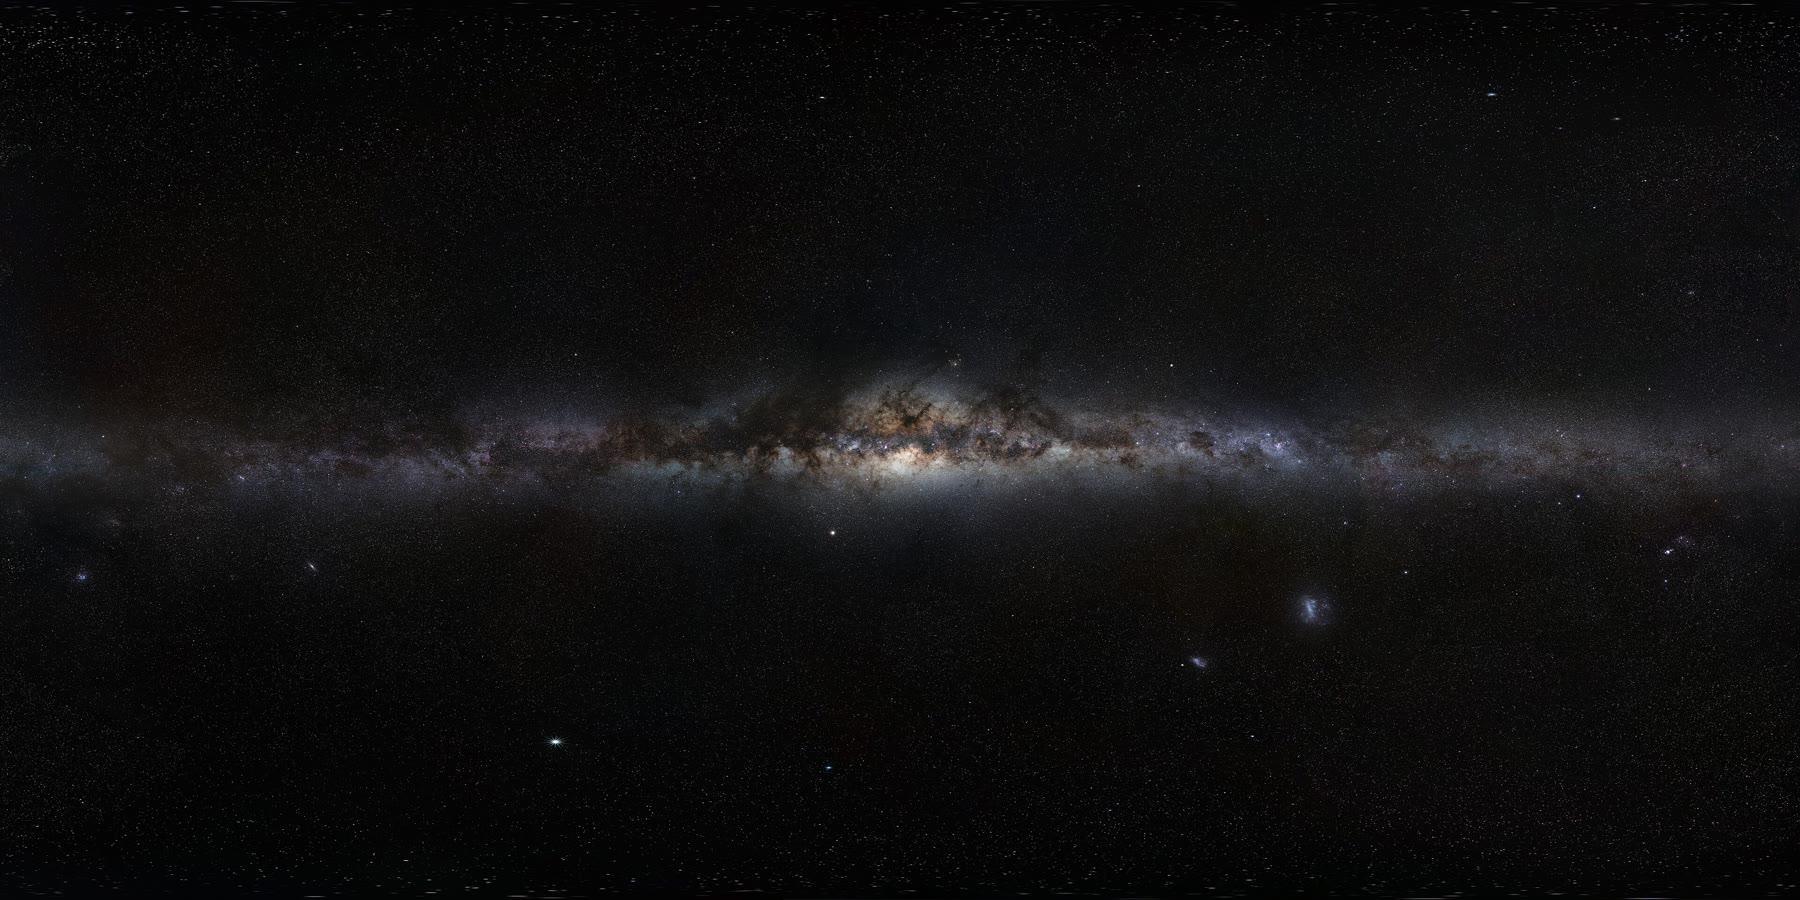
\includegraphics[width=0.96\linewidth]{images/book5/b3-milky-way-panorama.jpg}
\par\smallskip{\small 整个天空合成于一幅图像，投影使银河平面
横贯画面中部，其中心位于画面正中。光带是从内部所见的盘面，
暗色条纹是盘面中的尘埃，遮挡了其后的恒星；
中央的核球在中心周围隆起。光带下方靠右的两个小斑块，
即大、小麦哲伦云；
两者均为卫星星系。光带下方靠近左边缘的淡弱云斑，
是仙女座星系。
照片：ESO/S.~Brunier, CC BY~4.0。}\label{fig:b3:milky-way-galaxies:panorama}
\end{omfigure}
% ledger: photo:b3-milky-way-panorama, mcconn12:local-group

\begin{definition}[银盘、厚盘、银河系核球与恒星晕]\label{def:b3:milky-way-galaxies:structure}
称\emph{银盘}\index{银盘}为银河系中扁平的组分，
由恒星、气体和尘埃组成，近似圆轨道绕其
中心运行；其密度随离中央面的高度大致按指数规律下降，
并随离中心的距离而下降，尺度为一个标高和一个
标长。称\emph{厚盘}\index{厚盘}为第二个较老的盘状组分，
其标高较大、质量较小。称
\emph{银河系核球}\index{银河系核球}为从盘面中隆起的恒星中心密集区，
即向外突出的部分。称\emph{恒星晕}\index{恒星晕}
为稀疏、近似球形的老年恒星和球状星团组分，
环绕着盘面和核球。
\end{definition}

银河系是一个棒旋星系。在太阳附近，薄盘的
标高约为 \qty{300}{pc}，\omterm{def:b3:milky-way-galaxies:structure}{厚盘}的标高约为
\qty{900}{pc}；二者的标长分别约为 \qty{2.6}{kpc} 和
\qty{2.0}{kpc}。\omterm{def:b3:milky-way-galaxies:structure}{厚盘}包含约 \num{6e9} 个太阳质量，
约为薄盘的五分之一。从侧面看，核球呈箱形
或花生状：它是恒星棒向内加厚的部分，该棒的
半长约 \qty{5}{kpc}，其长轴与太阳至中心的连线成
\ang{27} 的夹角。\omterm{def:b3:milky-way-galaxies:structure}{恒星晕}所含恒星仅
约占百分之一。合计，银河系的恒星总质量约为
\num{5e10} 个太阳质量。
% ledger: bhg16:structure

\begin{omfigure}
\centering
\begin{tikzpicture}[x=0.17cm, y=0.17cm, font=\scriptsize]
% edge-on view
\begin{scope}
\fill[omProp!8] (0,0) circle (17);
\draw[omProp!60, densely dotted] (0,0) circle (17);
\fill[black!12] (0,0) ellipse (15 and 2.4);
\fill[black!30] (0,0) ellipse (15 and 0.8);
\fill[black!45] (-3.2,0) .. controls (-3.4,2.3) and (-1.2,2.0) .. (0,1.4)
  .. controls (1.2,2.0) and (3.4,2.3) .. (3.2,0)
  .. controls (3.4,-2.3) and (1.2,-2.0) .. (0,-1.4)
  .. controls (-1.2,-2.0) and (-3.4,-2.3) .. (-3.2,0) -- cycle;
\foreach \p in {(-10,9),(6,12),(12,-7),(-6,-13),(-13,-4),(3,-9),(12,8)}
  \fill[omProp] \p circle (0.35);
\fill[ocYellow, draw=black] (-8.2,0.15) circle (0.55);
\node[anchor=south] at (-8.2,0.9) {太阳};
\draw[|<->|] (0,-4.6) -- node[below] {$R_0 \approx \qty{8.2}{kpc}$} (-8.2,-4.6);
\node[anchor=west] at (15.3,0) {薄盘};
\node[anchor=west] at (13.2,2.8) {厚盘};
\draw[->] (4.6,4.6) node[anchor=south west, inner sep=1pt] {核球} -- (2.4,1.7);
\node[omProp!80!black] at (-11,13.5) {恒星晕};
\node at (0,-19.5) {(a) 侧视};
\end{scope}
% face-on view
\begin{scope}[xshift=7.6cm]
\fill[omProp!8] (0,0) circle (17);
\draw[omProp!60, densely dotted] (0,0) circle (17);
\fill[black!12] (0,0) circle (15);
\foreach \a in {0,180} {
  \draw[line width=1.6pt, black!40, rotate=\a+63]
    plot[domain=0:3.9, samples=50] ({5*exp(0.25*\x)*cos(\x r)}, {5*exp(0.25*\x)*sin(\x r)});
}
\fill[black!45, rotate=63] (0,0) ellipse (5 and 1.5);
\draw[dashed] (0,0) circle (8.2);
\fill[ocYellow, draw=black] (0,-8.2) circle (0.55);
\node[anchor=north] at (0,-8.9) {太阳};
\draw[dotted, thick] (0,0) -- (0,-8.2);
\draw[thick, ->] (0,0) ++(25:16) arc (25:-25:16);
\node[anchor=west] at (17.3,0) {自转};
\node[anchor=west, fill=black!12, inner sep=1pt] at (3.4,3.4) {棒};
\draw[|-|] (6,-15.5) -- node[below] {\qty{5}{kpc}} (11,-15.5);
\node at (0,-19.5) {(b) 从北银极所见};
\end{scope}
\end{tikzpicture}
\par\smallskip{\small 银河系示意图，按比例绘出其主要
尺度。(a)~侧视：薄盘（深色带）、\omterm{def:b3:milky-way-galaxies:structure}{厚盘}（浅色带）
、箱形核球，以及带有
球状星团（橙色点）的\omterm{def:b3:milky-way-galaxies:structure}{恒星晕}；太阳位于盘面中，距中心约 \qty{8.2}{kpc}，
并位于中央面之上约 \qty{25}{pc}（图中太小，
无法显示）。(b)~从北银极所见：棒，半长约
\qty{5}{kpc}，相对太阳至中心的连线倾斜 \ang{27}
（点线）；太阳圈（虚线）；
旋臂为示意画法；银河系在此视图中顺时针转动。}\label{fig:b3:milky-way-galaxies:sketch}
\end{omfigure}
% ledger: bhg16:structure, gravity19:r0

\begin{definition}[星族]\label{def:b3:milky-way-galaxies:populations}
\emph{星族}\index{星族}是指星系中
具有一定年龄范围、化学组成范围和轨道范围的一群恒星。
薄盘中的年轻恒星富含比氦重的元素，
轨道近似为圆形，传统上称为星族~I；
晕和球状星团中的老年恒星，重元素贫乏，
轨道上随机运动较大、净自转很小，
称为星族~II。
\end{definition}

\omterm{def:b3:milky-way-galaxies:structure}{厚盘}介于两者之间：其恒星大多比薄盘中的恒星年老，
在铁含量相同时，富含较轻的元素，
天文学家称之为 α 元素，以铁为基准度量。
\omterm{def:b3:milky-way-galaxies:structure}{恒星晕}是一份
化石记录：其中大部分由曾落入银河系、
被其潮汐撕碎的小星系聚集而成，其中一些恒星流
至今仍可在天空中追踪。
% ledger: bhg16:populations

\begin{definition}[银道坐标]\label{def:b3:milky-way-galaxies:coordinates}
某方向的\emph{银道坐标}\index{银道坐标}包括：
\emph{银纬} $b$，即该方向与银道面的夹角
（向北银极一侧为正）；以及\emph{银
经} $\ell$，在银道面内从银心方向
（$\ell = 0$）起算，经 $\ell = \ang{90}$，
即银河系自转带动太阳运动的方向。银道面于
1958 年确定，取为银河系中性氢的主平面；
北银极的赤经为 \ang{192.25}
（$12^\mathrm{h}49^\mathrm{m}$），赤纬为 \ang{27.4}（历元
1950）。
\end{definition}
% ledger: liu11:galactic, reid20:sgra

太阳并不恰在银道面上：它位于其北侧约 \qty{25}{pc} 处。
它到银心的距离 $R_0$ 曾长期是
银河天文学中最不确定的数值。现在它已由几何方法测得：恒星 S2 绕
银河系中心黑洞运行，周期为 \num{16}~年；其
在天空中的视角大小，以及沿\omterm{def:b3:remote-sensing-gis:insar}{视线方向}的速度，经
过 27 年跟踪，可直接给出到银心的距离：
$R_0 = \qty{8178}{pc}$，统计误差为 \qty{13}{pc}，
系统误差为 \qty{22}{pc}。综合各种方法的结果，
得 $R_0 = \qty[separate-uncertainty=true]{8.2 \pm 0.1}{kpc}$。
% ledger: bhg16:structure, gravity19:r0

\section{自转与暗物质晕}\label{sec:b3:milky-way-galaxies:rotation}

\begin{definition}[本地静止标准]\label{def:b3:milky-way-galaxies:lsr}
\emph{本地静止标准}\index{本地静止标准}（LSR）是这样一个参考系，
它沿通过太阳当前位置的、绕银心的圆轨道运动，
附近恒星和气体的速度
都相对于它给出。
\end{definition}

太阳相对于 LSR 大约以 \qty{10}{km.s^{-1}} 的速度指向银心运动，
以 \qty{11}{km.s^{-1}} 的速度沿自转方向运动，
并以 \qty{7}{km.s^{-1}} 的速度指向北银极运动：
这是叠加在轨道运动之上的一个小小的本动，轨道速度 $V_0$
约为数百千米每秒。从地球上看，银河系中心的射电源
沿银道面每年漂移 \qty{6.411}{mas}；这一漂移几乎全部
来自太阳轨道运动的反射，由此可得太阳绕银心的总速度
为 \qty[separate-uncertainty=true]{248 \pm 3}{km.s^{-1}}
（见\cref{exo:b3:milky-way-galaxies:2}）。
% ledger: bhg16:lsr, reid20:sgra

\begin{definition}[自转曲线；奥尔特常数]\label{def:b3:milky-way-galaxies:rotation-curve}
盘状星系的\emph{自转曲线}\index{自转曲线}是圆轨道在其盘面内的速度
$V(R)$ 随到其中心距离 $R$ 的变化关系。
对银河系，记 $V_0 = V(R_0)$，
$V'_0 = \mathrm{d}V/\mathrm{d}R$ 在 $R_0$ 处取值，则\emph{奥尔特
常数}\index{奥尔特常数}为
\[
A = \frac12\left(\frac{V_0}{R_0} - V'_0\right), \qquad
B = -\frac12\left(\frac{V_0}{R_0} + V'_0\right).
\]
\end{definition}

$A$ 度量盘的自转剪切，$B$ 度量其涡度：若盘像刚体一样转动，
则 $V'_0 = V_0/R_0$，$A = 0$；对平坦的
\omterm{def:b3:milky-way-galaxies:rotation-curve}{自转曲线}，$A = -B$。二者之差为 LSR 的角速度，
$A - B = V_0/R_0 = \omega_0$，二者之和为斜率，$A + B = -V'_0$。

\begin{theorem}[奥尔特公式]\label{thm:b3:milky-way-galaxies:oort}
银道面内距太阳 $d \ll R_0$ 处的一颗恒星，
银经为 $\ell$，做圆轨道运动，相对于 LSR 的径向
速度 $v_r$ 与切向速度 $v_t$（以
$\ell$ 增大的方向为正）。由下式给出：
\[
v_r = A\,d\sin 2\ell, \qquad v_t = d\,(A\cos 2\ell + B),
\]
在 $d/R_0$ 的一阶近似下成立。
\end{theorem}

\begin{proof}
设 $\omega(R) = V(R)/R$ 为 $R$ 处轨道的角速度。
取银心为原点，太阳位于距离 $R_0$ 处，
设恒星到银心的距离为 $R$，从银心看恒星的位置
与太阳位置的夹角为 $\theta$。
将恒星速度 $\omega R$ 与 LSR 速度 $\omega_0 R_0$ 投影到\omterm{def:b3:remote-sensing-gis:insar}{视线方向}，
利用太阳–恒星–银心三角形中的简单三角关系（
正弦定理给出 $R\sin(\ell + \theta) = R_0\sin\ell$），得精确结果
$v_r = R_0\,[\omega(R) - \omega_0]\sin\ell$。同理，
在与视线垂直的方向上，
$v_t = R_0\,[\omega(R) - \omega_0]\cos\ell - \omega(R)\,d$。对近邻恒星，
$\omega(R) - \omega_0 \approx \omega'_0\,(R - R_0)$，且
$R - R_0 \approx -d\cos\ell$。于是
$v_r \approx -R_0\omega'_0\,d\cos\ell\sin\ell = -\tfrac12 R_0\omega'_0\,
d\sin 2\ell$，保留一阶项，
$v_t \approx -R_0\omega'_0\,d\cos^2\ell - \omega_0 d$。
代入 $\omega'_0 = V'_0/R_0 - V_0/R_0^2$，$-\tfrac12 R_0\omega'_0 = A$，且
$-R_0\omega'_0\cos^2\ell - \omega_0 = A(1 + \cos 2\ell) - (A - B) =
A\cos 2\ell + B$。
\end{proof}

因此，近邻恒星的径向速度随天空方向按 $\sin 2\ell$ 变化，
其自行则按 $\cos 2\ell$ 变化，平均值由 $B$ 决定。
由第一版 Gaia 星表中 \num{304267} 颗恒星的自行与视差，
取典型距离 \qty{230}{pc}，得到\omterm{def:b3:milky-way-galaxies:rotation-curve}{奥尔特常数}为
$A = \qty[separate-uncertainty=true]{15.3 \pm 0.4}{km.s^{-1}.kpc^{-1}}$
和 $B = \qty[separate-uncertainty=true]{-11.9 \pm 0.4}{km.s^{-1}.kpc^{-1}}$。
另有两个轴对称圆盘所不应具有的项，记为 $C$
与 $K$，其值约为 \qty{-3}{km.s^{-1}.kpc^{-1}}：局部圆盘
受棒状结构和旋臂的扰动。
% ledger: bovy17:oort

\subsection*{由 21 厘米谱线得到的自转曲线}

中性氢充满圆盘，并发射 21 厘米谱线，
其频率为 \qty{1420.405751}{MHz}；射电波能穿过在可见光波段遮蔽远处圆盘的
尘埃。沿盘面内的一条\omterm{def:b3:remote-sensing-gis:insar}{视线方向}，
每团气体都在其径向速度所对应的多普勒频移处
贡献一条谱线，谱线的轮廓即为速度谱。
在太阳圆之内，唯有一个速度被单独突出。
% ledger: nrao:hi-line

\begin{theorem}[切点法]\label{thm:b3:milky-way-galaxies:tangent}
设气体沿圆轨道运动，其角速度 $\omega(R)$
随向外距离增大而减小。沿经度
$0 < \ell < \ang{90}$ 的\omterm{def:b3:remote-sensing-gis:insar}{视线方向}，相对于\omterm{def:b3:milky-way-galaxies:lsr}{本地静止标准}的径向速度
在切点处最大，切点即\omterm{def:b3:remote-sensing-gis:insar}{视线方向}与某一轨道相切之处，位于
$R = R_0\sin\ell$ 处，其最大值为
\[
v_\mathrm{max} = V(R_0\sin\ell) - V_0\sin\ell .
\]
\end{theorem}

\begin{proof}
由奥尔特公式的证明可知，\omterm{def:b3:remote-sensing-gis:insar}{视线方向}上距中心为 $R$ 的气体
有 $v_r = R_0\,[\omega(R) - \omega_0]\sin\ell$。由于
$\sin\ell > 0$ 且 $\omega$ 递减，$v_r$ 在 $R$
最小处最大。沿\omterm{def:b3:remote-sensing-gis:insar}{视线方向}，$R$ 在自中心所作视线垂线的
垂足处最小，此处 $R = R_0\sin\ell$。
于是 $R_0\,\omega(R)\sin\ell = \omega(R)\,R = V(R)$，且
$R_0\,\omega_0\sin\ell = V_0\sin\ell$。
\end{proof}

\begin{omfigure}
\centering
\begin{tikzpicture}[scale=0.95, font=\small]
\coordinate (C) at (0,0);
\coordinate (S) at (0,-4);
\coordinate (T) at (-1.970,-1.653);
\draw[dashed, black!50] (C) circle (4);
\draw[dashed, omDef!70] (C) circle (2.571);
\fill (C) circle (2pt) node[anchor=south west] {银心};
\fill[ocYellow, draw=black] (S) circle (3pt);
\node[anchor=north] at (0,-4.15) {太阳};
\draw[thick] (S) -- ($(S)!2.25!(T)$) node[anchor=south east, fill=white, inner sep=1pt] {视线方向};
\draw[dotted, thick] (C) -- (S);
\draw[thick, omThm] (C) -- node[anchor=north west, fill=white, inner sep=1pt, pos=0.45] {$R_0\sin\ell$} (T);
\fill[omThm] (T) circle (2pt);
\node[anchor=north east, omThm, fill=white, inner sep=1pt] at ($(T)+(-0.05,-0.08)$) {切点};
\draw[->, very thick, omDef] (T) -- ++(-0.643*1.3, 0.766*1.3) node[anchor=south west, fill=white, inner sep=1pt] {$V(R)$};
\draw[->, very thick, black!70] (S) -- ++(-1.4,0) node[anchor=north] {$V_0$};
\draw (0,-3.2) arc (90:130:0.8);
\node at (-0.30,-2.85) {$\ell$};
\node[anchor=west] at (0.1,-2.2) {$R_0$};
\node[black!60, anchor=west] at (2.9,-2.9) {太阳圆};
\end{tikzpicture}
\par\smallskip{\small 切点法示意图，自北银极向下看。
沿经度为 $\ell$ 的\omterm{def:b3:remote-sensing-gis:insar}{视线方向}，离银心最近的气体
位于切点处，$R = R_0\sin\ell$（红色）；其轨道速度 $V(R)$
沿\omterm{def:b3:remote-sensing-gis:insar}{视线方向}，切点处的径向速度即谱线轮廓所示的
最大值。每个
经度给出太阳圆之内\omterm{def:b3:milky-way-galaxies:rotation-curve}{自转曲线}上的一个点。}\label{fig:b3:milky-way-galaxies:tangent}
\end{omfigure}

因此，每条 21 厘米谱线轮廓中的最大速度给出 $V$
在 $R_0\sin\ell$ 处的值，经度从 \ang{0} 扫至 \ang{90}，
便得到从银心到太阳的\omterm{def:b3:milky-way-galaxies:rotation-curve}{自转曲线}。太阳圆之外
没有\omterm{def:b3:remote-sensing-gis:insar}{视线方向}与轨道相切，此法失效：
此时必须同时测定每个示踪天体的距离及其
速度。自 2014 年以来，一颗卫星已测得逾 10 亿颗恒星的视差，
外侧\omterm{def:b3:milky-way-galaxies:rotation-curve}{自转曲线}如今由恒星示踪。
% ledger: nrao:hi-line, gaia:dr3

\begin{omfigure}
\centering
\begin{tikzpicture}
\begin{axis}[width=0.90\linewidth, height=0.52\linewidth,
  xmin=0, xmax=26, ymin=0, ymax=265,
  xlabel={距银心距离 $R$（kpc）}, ylabel={圆轨道速度（\unit{km.s^{-1}}）},
  tick label style={font=\scriptsize}, label style={font=\small},
  legend style={font=\scriptsize, at={(0.5,-0.16)}, anchor=north, legend columns=4, draw=none, cells={anchor=west}, /tikz/every even column/.append style={column sep=1em}}]
\addplot[thin, black!40, dashed, forget plot] coordinates {(8.122,0) (8.122,265)};
\node[font=\scriptsize, anchor=south west, rotate=90] at (axis cs:7.9,4) {太阳};
\addplot[only marks, mark=*, mark size=1.1pt, black, error bars/.cd, y dir=both, y explicit]
  table[x=R, y=vc, y error minus=sig_lo, y error plus=sig_hi] {figdata/out/bachelor-3-rotation_curve-data.dat};
\addlegendentry{实测}
\addplot[very thick, omDef] table[x=R, y=v_tot] {figdata/out/bachelor-3-rotation_curve-model.dat};
\addlegendentry{模型总和}
\addplot[thick, black!55] table[x=R, y=v_bar] {figdata/out/bachelor-3-rotation_curve-model.dat};
\addlegendentry{全部重子}
\addplot[thick, dashed, red!70!black] table[x=R, y=v_halo] {figdata/out/bachelor-3-rotation_curve-model.dat};
\addlegendentry{暗物质晕}
\addplot[densely dotted, thick, omProp] table[x=R, y=v_bulge] {figdata/out/bachelor-3-rotation_curve-model.dat};
\addlegendentry{核球}
\addplot[dashdotted, thick, omMeth] table[x=R, y=v_thin] {figdata/out/bachelor-3-rotation_curve-model.dat};
\addlegendentry{薄盘}
\addplot[densely dashed, thick, violet!70!black] table[x=R, y=v_thick] {figdata/out/bachelor-3-rotation_curve-model.dat};
\addlegendentry{厚盘}
\end{axis}
\end{tikzpicture}
\par\smallskip{\small 银河系的\omterm{def:b3:milky-way-galaxies:rotation-curve}{自转曲线}。圆点：
由 5 至 \qty{25}{kpc} 之间的红巨星测得的圆轨道速度（Eilers
等，2019），附误差棒。曲线为
某一已发表质量模型中核球、薄盘与\omterm{def:b3:milky-way-galaxies:structure}{厚盘}
单独给出的速度（Pouliasis 等，2017），其合成（灰色），以及
此处拟合到观测数据的\omterm{def:b3:milky-way-galaxies:halo}{暗物质晕}（红色虚线），它
在 \qty{14}{kpc} 之外接替重子；各分量按平方和方式合成为
总速度（蓝色）。内部 \qty{5}{kpc}，因棒状结构使轨道
远非圆形，未纳入测量。}\label{fig:b3:milky-way-galaxies:rotation}
\end{omfigure}
% ledger: eilers19:table1, eilers19:vc, eilers19:halo, pouliasis17:model1, data:b5-rotation-fit

上图中的曲线，是依据超过两万三千颗明亮红巨星的
位置、距离与速度测得的，
所用的是恒星流体动力学中的方程，它把一群恒星的平均运动与
维系它们的引力联系起来（金斯方程）。
在太阳处，它给出 $V_0 = \qty{229.0}{km.s^{-1}}$，系统不确定度为百分之二至五；
更远处则缓慢下降，每千秒差距下降
\qty[separate-uncertainty=true]{1.7 \pm 0.1}{km.s^{-1}}。它
并不像可见质量所要求的那样下降。
% ledger: eilers19:vc

\subsection*{银河系质量的测定}

圆盘的引力并非球体的引力，但质量模型的速度曲线
在每个分量的势可写成闭合形式时，便易于算出。
下面平面中的势，取自一个已发表的
银河系恒星模型。

\begin{proposition}[三种质量模型的圆轨道速度]\label{prop:b3:milky-way-galaxies:models}
在平面 $z = 0$ 上，圆轨道速度 $V^2 = R\,\partial\Phi/\partial R$
对以下各种情形分别为：
\begin{itemize}
\item 质量为 $M$、核半径为 $b$ 的普默尔球，其势为
  $\Phi = -GM/\sqrt{r^2 + b^2}$：
  \[ V^2 = \frac{GMR^2}{(R^2 + b^2)^{3/2}}\,; \]
\item 宫本–永井圆盘，质量为 $M$，标长为 $a$，
  标高为 $b$，其势为
  $\Phi = -GM\big/\sqrt{R^2 + \bigl(a + \sqrt{z^2 + b^2}\,\bigr)^2}$：
  \[ V^2 = \frac{GMR^2}{\bigl(R^2 + (a + b)^2\bigr)^{3/2}}\,; \]
\item 纳瓦罗–弗伦克–怀特晕，其密度为
  $\rho = \rho_0\big/\bigl[x(1 + x)^2\bigr]$，$x = r/R_s$；半径 $r$ 以内的质量
  为 $M(r) = 4\pi\rho_0R_s^3\bigl[\ln(1 + x) - x/(1 + x)\bigr]$，且
  $V^2 = GM(r)/r$。
\end{itemize}
若有多个分量，则各分量速度的平方相加。
\end{proposition}

\begin{proof}
对前两式，对势关于 $R$ 求导，
在 $z = 0$ 处取值。对于晕，将 $4\pi r^2\rho$ 从 0 到 $r$ 积分，并取
$u = 1 + x'$，$\int_0^x x'\,\mathrm{d}x'/(1 + x')^2 =
\int_1^{1+x}(u - 1)\,\mathrm{d}u/u^2 = \ln(1 + x) + 1/(1 + x) - 1$；
球对称质量作用于 $r$ 处轨道，如同其 $r$ 以内
的全部质量都集中于中心（牛顿定理）。势可相加，
因而其径向导数亦相加。
\end{proof}

图中所用的模型包含一个普默尔核球，其质量为
\num{1.07e10} 个太阳质量，$b = \qty{0.3}{kpc}$，另有一个薄盘与一个
\omterm{def:b3:milky-way-galaxies:structure}{厚盘}，各自质量为 \num{3.94e10} 个太阳质量，参数 $(a, b) =
(\qty{5.3}{kpc}, \qty{0.25}{kpc})$ 与 $(\qty{2.6}{kpc}, \qty{0.8}{kpc})$。
取 $G = \qty{4.301e-6}{kpc.(km.s^{-1})^2}$（每太阳质量），则其恒星
单独给出的太阳轨道速度为 \qty{184}{km.s^{-1}}，而
位于 \qty{20}{kpc} 处的恒星为 \qty{134}{km.s^{-1}}；实测速度分别为
229 与 \qty{200}{km.s^{-1}}。以实测数据拟合的晕，在恒星保持固定时，
具有 $R_s = \qty{14.75}{kpc}$ 与
$\rho_0 = \num{1.06e7}$ 太阳质量每立方千秒差距，与
作者所拟合的晕相同（$R_s = \qty[separate-uncertainty=true]{14.8 \pm 0.4}{kpc}$，
$\rho_0 = \qty[separate-uncertainty=true]{1.06 \pm 0.09 e7}{}$ 太阳质量
每立方千秒差距）。晕在约 \qty{14}{kpc} 之外占主导。
% ledger: pouliasis17:model1, data:b5-rotation-fit, eilers19:halo, eilers19:table1, const:G, sun:mass, iau:parsec

\begin{definition}[暗物质晕]\label{def:b3:milky-way-galaxies:halo}
星系的\emph{暗物质晕}\index{暗物质晕}是
大致呈球状分布的暗物质，其中嵌有恒星与气体，
其尺度与质量都远大于可见组分，
其存在由引力推断得出：由\omterm{def:b3:milky-way-galaxies:rotation-curve}{自转曲线}，由
卫星星系与晕星的运动，以及由光线的弯曲。
\end{definition}

\begin{theorem}[半径以内的质量]\label{thm:b3:milky-way-galaxies:enclosed}
对于球对称质量分布，半径 $r$ 处的圆轨道速度
给出其内的质量 $M(r) = rV^2/G$。平坦的\omterm{def:b3:milky-way-galaxies:rotation-curve}{自转曲线}，
若 $V = $ 常数，则蕴含 $M(r) \propto r$，且
密度为 $\rho(r) = V^2/(4\pi G r^2)$。
\end{theorem}

\begin{proof}
由牛顿定理，半径 $r$ 处的引力为 $GM(r)/r^2$，它提供
圆轨道所需的向心加速度 $V^2/r$。若 $V$ 为常数，
则 $\mathrm{d}M/\mathrm{d}r = V^2/G = 4\pi r^2\rho$。
\end{proof}

对于扁平的圆盘，$rV^2/G$ 并非严格等于 $r$ 以内的质量，但
它是球体产生同一轨道所需的质量，并且
此处按惯例将其用作\emph{动力学质量}。下图
将其与恒星及整个银河系进行比较。

\begin{omfigure}
\centering
\begin{tikzpicture}
\begin{axis}[width=0.80\linewidth, height=0.50\linewidth,
  xmin=0, xmax=30, ymin=0, ymax=28,
  xlabel={半径 $R$ (kpc)}, ylabel={$RV^2/G$（$10^{10}$ 太阳质量）},
  tick label style={font=\scriptsize}, label style={font=\small},
  legend style={font=\scriptsize, at={(0.03,0.97)}, anchor=north west, draw=none, fill=white, cells={anchor=west}}]
\addplot[very thick, omDef] table[x=R, y=m_tot] {figdata/out/bachelor-3-rotation_curve-mass.dat};
\addlegendentry{总量，模型}
\addplot[only marks, mark=*, mark size=1.1pt, black] table[x=R, y=m_dyn] {figdata/out/bachelor-3-rotation_curve-mdata.dat};
\addlegendentry{总量，由实测速度得到}
\addplot[thick, black!55] table[x=R, y=m_bar] {figdata/out/bachelor-3-rotation_curve-mass.dat};
\addlegendentry{恒星，模型}
\end{axis}
\end{tikzpicture}
\par\smallskip{\small 动力学质量 $RV^2/G$，指半径 $R$ 以内的部分。
可见质量约在 $9\times10^{10}$ 太阳质量处趋于平稳，此即
模型中核球与圆盘的质量；总量则几乎按
与 $R$ 成正比增长，正如平坦\omterm{def:b3:milky-way-galaxies:rotation-curve}{自转曲线}所要求的。在
\qty{20}{kpc} 处，总量超过可见质量的两倍。}\label{fig:b3:milky-way-galaxies:mass}
\end{omfigure}
% ledger: data:b5-rotation-fit, eilers19:table1, pouliasis17:model1

暗晕延伸多远、总质量多大，仅凭盘的
\omterm{def:b3:milky-way-galaxies:rotation-curve}{自转曲线}无法说明。用测量作者拟合的轮廓外推到
其维里半径（约 \qty{190}{kpc}）处，测量作者拟合的暗晕
约含 \num{7e11} 太阳质量；一篇对其他估计的综述则给出 \num{1.3e12}，
其中重子仅占约百分之七。太阳附近的暗物质很稀薄，
每立方厘米的质能约为 \qty{0.30}{GeV}，
相当于质子质量的三分之一，
因此它只通过累积的引力被感受到。
% ledger: eilers19:halo, bhg16:structure, nist:mp

\section{星系}\label{sec:b3:milky-way-galaxies:galaxies}

\begin{definition}[哈勃序列；椭圆星系、透镜状星系、旋涡星系与不规则星系]\label{def:b3:milky-way-galaxies:types}
\emph{哈勃序列}\index{哈勃序列}按
外观对星系分类。\emph{椭圆星系}\index{椭圆星系}
（E 型）是光滑的恒星系统，亮度自中心向外稳定下降，
且没有盘；记为 E$n$，其中 $n = 10(1 - b/a)$，
$b/a$ 为表观轴比，类型从 E0（圆形）到 E7。
\emph{旋涡星系}\index{旋涡星系}具有带旋臂的盘，
旋臂环绕中央核球；按核球渐小、旋臂渐开、旋臂中星形成团块渐趋破碎的顺序，依次记为 Sa、Sb、Sc；
若中心有棒穿过，则记为 SBa、SBb、SBc。
\emph{透镜状星系}\index{透镜状星系}
（S0）有盘和核球，但没有旋臂。
\emph{不规则星系}\index{不规则星系}（Irr、Im）没有
有组织的结构。
\end{definition}

\begin{omfigure}
\centering
\begin{tikzpicture}[font=\small]
\def\spiralgal#1#2#3#4#5{% x, y, bulge radius, winding rate, bar half-length
  \begin{scope}[shift={(#1,#2)}]
    \fill[black!12] (0,0) circle (0.66);
    \pgfmathsetmacro{\rs}{max(#3,#5)}
    \pgfmathsetmacro{\th}{ln(0.62/\rs)/#4}
    \foreach \a in {0,180}
      \draw[line width=1.2pt, black!55, rotate=\a]
        plot[domain=0:\th, samples=40] ({\rs*exp(#4*\x)*cos(\x r)}, {\rs*exp(#4*\x)*sin(\x r)});
    \ifdim #5pt>0pt \fill[black!50] (0,0) ellipse (#5 and 0.07); \fi
    \fill[black!60] (0,0) circle (#3);
  \end{scope}}
\fill[black!40] (0,0) circle (0.55);
\fill[black!40] (1.6,0) ellipse (0.55 and 0.385);
\fill[black!40] (3.2,0) ellipse (0.55 and 0.165);
\fill[black!15] (4.9,0) ellipse (0.62 and 0.20);
\fill[black!45] (4.9,0) ellipse (0.24 and 0.16);
\draw[black!40] (5.65,0) -- (6.3,1.25);
\draw[black!40] (5.65,0) -- (6.3,-1.25);
\spiralgal{7.1}{1.25}{0.26}{0.16}{0}
\spiralgal{8.8}{1.25}{0.15}{0.28}{0}
\spiralgal{10.5}{1.25}{0.07}{0.45}{0}
\spiralgal{7.1}{-1.25}{0.20}{0.20}{0.34}
\spiralgal{8.8}{-1.25}{0.12}{0.32}{0.30}
\spiralgal{10.5}{-1.25}{0.06}{0.45}{0.26}
\foreach \p/\r in {(12.3,0.2)/0.22,(12.6,-0.15)/0.16,(12.05,-0.25)/0.12,(12.45,0.35)/0.1,(12.85,0.1)/0.13}
  \fill[black!35] \p circle (\r);
\foreach \x/\t in {0/E0,1.6/E3,3.2/E7,4.9/S0}
  \node at (\x,-0.95) {\t};
\foreach \x/\t in {7.1/Sa,8.8/Sb,10.5/Sc}
  { \node at (\x,0.35) {\t}; \node at (\x,-2.15) {SB\t}; }
\node at (12.45,-0.95) {不规则};
\node[font=\scriptsize, black!60] at (1.6,1.15) {椭圆星系};
\node[font=\scriptsize, black!60] at (4.9,1.15) {透镜状星系};
\node[font=\scriptsize, black!60] at (8.8,2.25) {旋涡星系};
\node[font=\scriptsize, black!60] at (8.8,-0.35) {棒旋星系};
\node[font=\scriptsize, black!60] at (12.45,1.15) {不规则星系};
\end{tikzpicture}
\par\smallskip{\small \omterm{def:b3:milky-way-galaxies:types}{哈勃序列}以音叉形式示意绘出，
\omterm{def:b3:milky-way-galaxies:types}{椭圆星系}按其表观扁率标注；
音叉在\omterm{def:b3:milky-way-galaxies:types}{透镜状星系}处分支为普通\omterm{def:b3:milky-way-galaxies:types}{旋涡星系}与棒旋星系，
二者均自大核球、紧绕旋臂（a）排列至
小核球、旋臂张开（c）；\omterm{def:b3:milky-way-galaxies:types}{不规则星系}收束整个序列。}\label{fig:b3:milky-way-galaxies:fork}
\end{omfigure}
% ledger: buta11:hubble

这些分类描述的是天上所见的形状，而同一个标签会掩盖一个
范围：沿最短轴观察的\omterm{def:b3:milky-way-galaxies:types}{椭圆星系}看上去总是圆的，
无论其真实扁率如何；相邻类别之间的界限也取决于判断。
在邻近星系的星表中，
银河系被列为 S(B)bc，即介于 Sb 与 Sc 之间的带棒\omterm{def:b3:milky-way-galaxies:types}{旋涡星系}；
其大邻居仙女座星系（M31）为 Sb，三角座星系（M33）为 Sc，
大、小麦哲伦云则是\omterm{def:b3:milky-way-galaxies:types}{不规则星系}。
% ledger: buta11:hubble, mcconn12:local-group

\begin{omfigure}
\centering
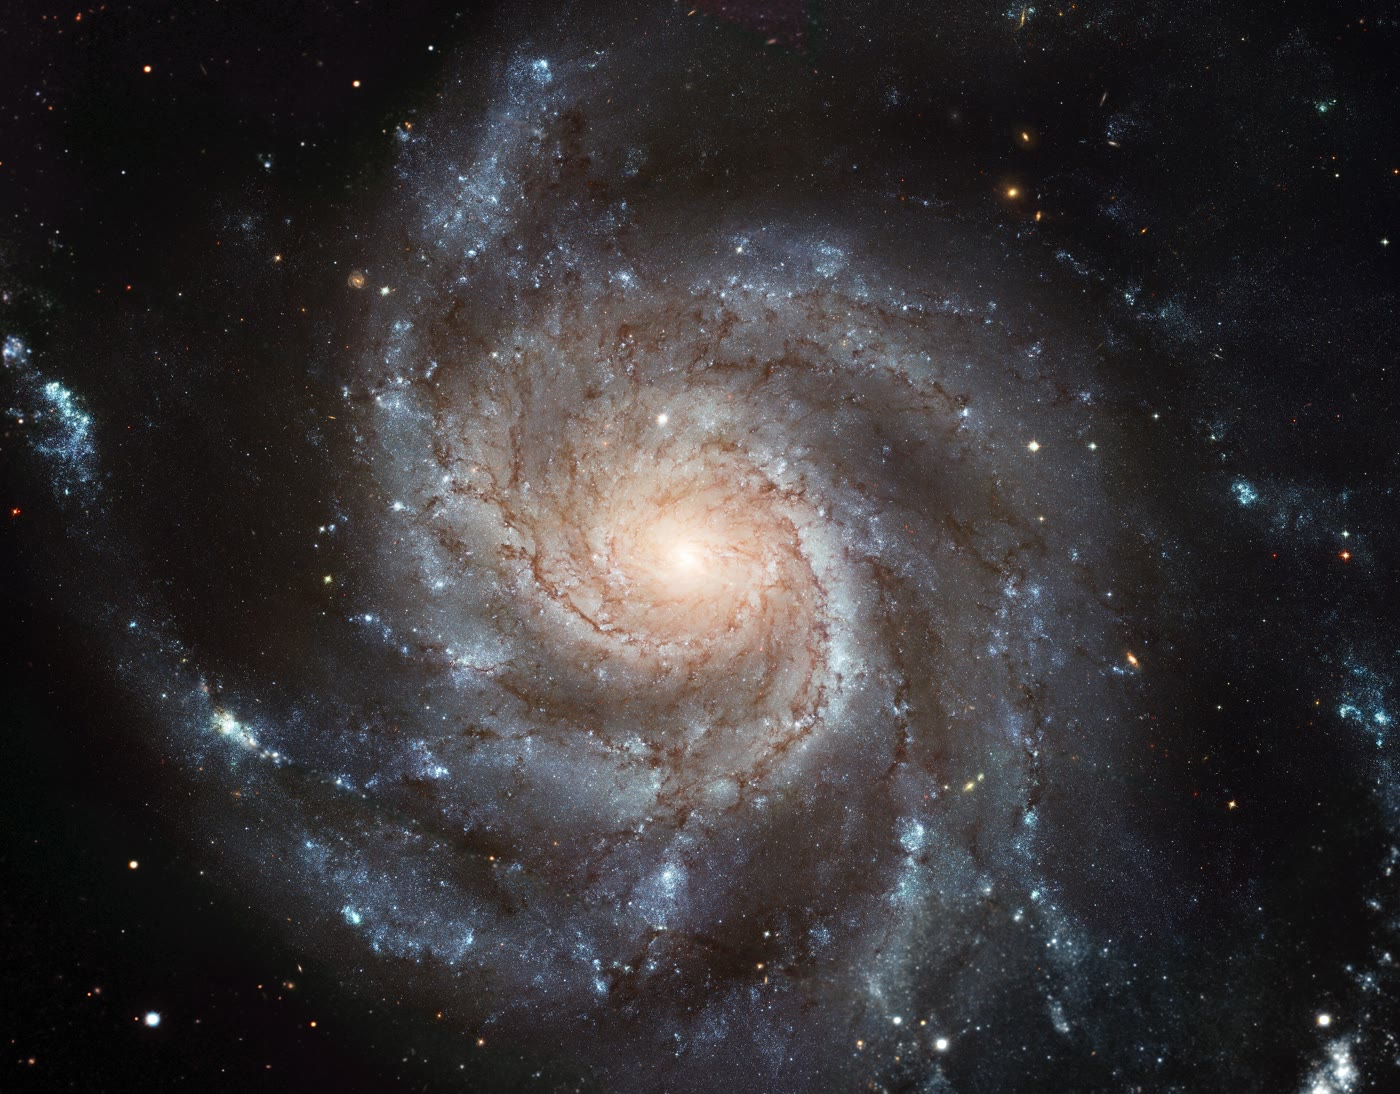
\includegraphics[width=0.66\linewidth]{images/book5/b3-m101.jpg}
\par\smallskip{\small 哈勃太空望远镜所拍摄的正面朝向\omterm{def:b3:milky-way-galaxies:types}{旋涡星系} M101，
由 51 次曝光拼接而成，边缘已裁剪：中央是一个小而明亮、略呈黄色的核球；
旋臂张开，颜色更蓝，并散布着年轻恒星团；
沿旋臂分布着褐色的尘埃带。图像：ESA 与 NASA
（Hubble, heic0602），CC BY~4.0。}\label{fig:b3:milky-way-galaxies:m101}
\end{omfigure}
% ledger: photo:b3-m101

旋臂为什么不会越绕越紧？在\omterm{def:b3:milky-way-galaxies:rotation-curve}{自转曲线}平坦的盘中，
离中心一半距离的恒星，绕行一周所需时间也只有一半。
若由恒星构成的旋臂随盘转动，每转一圈都会卷得更紧，
经过盘的几圈自转后，它就成了一团紧密的螺旋（见\cref{exo:b3:milky-way-galaxies:11}）。

\begin{definition}[密度波理论]\label{def:b3:milky-way-galaxies:density-wave}
\emph{密度波理论}\index{密度波理论}认为旋臂是盘中的一种高密度波，
即一种以自身角速度刚性转动的螺旋图样，其角速度称为图样速度，
而恒星与气体穿过这一图样运动，
进入拥挤的旋臂时减速，
离开时加速，如同汽车穿过交通堵塞路段一样。
\end{definition}

该理论于 1964 年提出，使旋臂摆脱了缠绕问题。
气体进入旋臂后被压缩，恒星便在此形成。旋臂
由年轻恒星与发光气体勾勒出来，而老年恒星则分布得
均匀得多。旋臂是否为长寿命的波，至今仍有争议；
盘的计算机模拟中更常见的是瞬变旋臂，
它们会消散又重新形成，而经过的星系或一根棒可以驱动
出双臂旋涡。
% ledger: dobbs14:density-wave

\begin{definition}[超大质量黑洞]\label{def:b3:milky-way-galaxies:smbh}
称\emph{超大质量黑洞}\index{超大质量黑洞}为位于星系中心的
质量达一百万个太阳质量或更大的黑洞。
\end{definition}

银河系中心的致密射电源人马座~A*
（Sgr~A*）周围有恒星沿紧致、快速的轨道运动，这些轨道要求
中心质量约为四百万个太阳，据对测量结果的综述为 $\num[separate-uncertainty=true]{4.2 \pm 0.2 e6}$
太阳质量。Sgr~A* 相对于遥远星系几乎不动：扣除太阳的运动后，
其残余运动至多每秒几千米，因此它至少
持有该质量的四分之一。其大小与
施瓦西半径相当，其密度超过 \num{4e23} 个太阳质量每立方秒差距，
与黑洞所预期的密度非常接近，
可见 Sgr~A* 是黑洞的
证据十分充分。
% ledger: reid20:sgra, bhg16:structure, gravity19:r0

\begin{definition}[本星系群；星系团]\label{def:b3:milky-way-galaxies:groups}
称\emph{本星系群}\index{本星系群}为由银河系和仙女座星系主导的
引力束缚星系群，两者各有其伴星系。
称\emph{星系团}\index{星系团}为最大的引力束缚系统之一：
许多星系与辐射 X 射线的热气体
一起被束缚在共同的引力势阱中，该势阱
主要由暗物质构成。
\end{definition}

距太阳 \qty{3}{Mpc} 之内有一百多个星系，其中
大多数是矮星系。大麦哲伦云距离约 \qty{50}{kpc}，仙女座星系距离
约为 \qty{783}{kpc}，并以 \qty{300}{km.s^{-1}} 的速度向我们靠近，\omterm{def:b3:milky-way-galaxies:groups}{本星系群}的束缚成员
大致位于距其质心 \qty{1.06}{Mpc} 以内，
位于银河系与仙女座星系之间，它们在那里脱离了宇宙的膨胀。
其质量由两大星系相互趋近的运动可得，
量级约为 \num{5e12} 个太阳质量。在大质量\omterm{def:b3:milky-way-galaxies:groups}{星系团}中，热气体温度约为 \qty{e8}{K}，
其质量约为恒星质量的十倍；星系与气体之和
相对于引力势阱的深度而言过轻，
\omterm{def:b3:milky-way-galaxies:groups}{星系团}的大部分质量，量级为 \num{e15} 个太阳质量，
是暗物质。
% ledger: mcconn12:local-group, kravtsov12:clusters

\section{距离阶梯}\label{sec:b3:milky-way-galaxies:ladder}

视差仅凭几何即可给出距离，但视差随距离增大而减小。
目前最好的视差星表测量了亮于星等~15 的恒星的视差，其
不确定度为 0.02 至 \qty{0.03}{mas}，因此可测出精度达 \qty{10}{\percent} 的距离，
适用范围约至 \qty{4}{kpc}；大麦哲伦云位于 \qty{50}{kpc}，
其视差为 \qty{0.02}{mas}。更远处的距离
只能依靠光度已知的天体
来确定。
% ledger: gaia:dr3, freedman19:trgb

\begin{definition}[标准烛光；距离阶梯]\label{def:b3:milky-way-galaxies:ladder}
称\emph{标准烛光}\index{标准烛光}为一类天体，其绝对星等已知，
或可由与距离无关地测得的性质推出，从而其视星等
给出距离模数。\emph{距离阶梯}\index{距离阶梯}是
一系列方法构成的链条，
每一级都在足够近、可由前一级方法同时测量的
天体上定标，
从而把距离由视差推广到膨胀的宇宙。
\end{definition}

\begin{definition}[造父变星；勒维特定律]\label{def:b3:milky-way-galaxies:cepheid}
称\emph{造父变星}\index{造父变星}为年轻、高光度、脉动的恒星，
其亮度以严格规则的周期变化，
周期约从一天到数周。\emph{勒维特定律}\index{勒维特定律}，
即周期–光度关系，是造父变星的平均绝对星等与其周期对数之间的
线性关系，
周期越长，恒星越亮。
\end{definition}

该关系于 1908 年在小麦哲伦云中发现，该星系中的恒星
距离几乎相同。宿主\omterm{def:b3:milky-way-galaxies:cepheid}{造父变星}的星系中的尘埃会使其变暗、变红；
但可见光波段的变暗量大于近红外波段，且其比值对给定类型的尘埃为定值，
因此选取 $W_I = I - 1.55\,(V - I)$ 作为组合，
即由 I 与 V 波段星等构成的韦森海特指数，其选取使变暗效应相互抵消。
下图给出大麦哲伦云中 2315 颗\omterm{def:b3:milky-way-galaxies:cepheid}{造父变星}的情况，
\omterm{def:b3:milky-way-galaxies:cepheid}{勒维特定律}在图中表现为一条紧密的直线，其散布为
\qty{0.078}{mag}，
相当于单颗恒星的距离误差
\qty{3.6}{\percent}。
% ledger: sos15:leavitt, data:b5-ogle-lmc-cep

\begin{omfigure}
\centering
\begin{tikzpicture}
\begin{axis}[width=0.80\linewidth, height=0.52\linewidth,
  xmin=-0.05, xmax=1.6, ymin=10, ymax=16.6, y dir=reverse,
  xlabel={$\log_{10}(P/\mathrm{d})$}, ylabel={韦森海特指数 $W_I$（星等）},
  tick label style={font=\scriptsize}, label style={font=\small},
  legend style={font=\scriptsize, at={(0.5,-0.17)}, anchor=north, legend columns=3, draw=none, cells={anchor=west}, /tikz/every even column/.append style={column sep=1em}},
  legend image post style={scale=2.2}]
\addplot[only marks, mark=*, mark size=0.45pt, omDef, opacity=0.6] table[x=logp, y=w] {figdata/out/bachelor-3-distance_ladder-pl.dat};
\addlegendentry{造父变星}
\addplot[only marks, mark=x, mark size=1.6pt, red!70!black] table[x=logp, y=w] {figdata/out/bachelor-3-distance_ladder-clipped.dat};
\addlegendentry{剔除（$>3\sigma$）}
\addplot[thick, black] table[x=logp, y=w_fit] {figdata/out/bachelor-3-distance_ladder-fit.dat};
\addlegendentry{拟合}
\node[font=\scriptsize, anchor=south west, fill=white, inner sep=1pt] at (axis cs:0.55,11.0) {$W_I = -3.315\log_{10}P + 15.889$};
\end{axis}
\end{tikzpicture}
\par\smallskip{\small 大麦哲伦云中的\omterm{def:b3:milky-way-galaxies:cepheid}{勒维特定律}：
2315 颗基模脉动\omterm{def:b3:milky-way-galaxies:cepheid}{造父变星}的韦森海特指数
对其周期对数作图（OGLE 巡天，Soszy\'nski 等，2015 年，经 CDS 获取）。
亮星位于上方。以最小二乘法拟合直线，
剔除偏离该直线超过三个标准差的 92 颗恒星后，
所得直线再现了已发表的关系（$-3.314$，$15.888$）。
取大麦哲伦云的距离模数 18.477，
该直线可由任一\omterm{def:b3:milky-way-galaxies:cepheid}{造父变星}的周期给出其绝对韦森海特星等。}\label{fig:b3:milky-way-galaxies:leavitt}
\end{omfigure}
% ledger: data:b5-ogle-lmc-cep, sos15:leavitt, freedman19:trgb

\begin{definition}[红巨星支顶端]\label{def:b3:milky-way-galaxies:trgb}
\emph{红巨星支顶端}\index{红巨星支顶端}
（TRGB）是某一古老\omterm{def:b3:milky-way-galaxies:populations}{星族}中红巨星光度的尖锐上限，
这一上限由其核心中氦的点燃所决定，
即氦闪；在 I 波段，它在各古老\omterm{def:b3:milky-way-galaxies:populations}{星族}中的绝对星等几乎相同，
$M_I \approx -4.05$，对应的颜色为
$V - I = 1.6$，且仅微弱地依赖于化学组成。
\end{definition}

\omterm{def:b3:milky-way-galaxies:trgb}{红巨星支顶端}在星系稀疏的晕中测量，那里尘埃少、星体拥挤程度低，
它使用古老的晕星，而\omterm{def:b3:milky-way-galaxies:cepheid}{造父变星}使用
年轻的盘星，二者所依据的物理并不相同。\omterm{def:b3:milky-way-galaxies:cepheid}{造父变星}与
\omterm{def:b3:milky-way-galaxies:trgb}{红巨星支顶端}可达几十兆秒差距，并能进入那些曾有罕见且亮得多的\omterm{def:b3:milky-way-galaxies:ladder}{标准烛光}
发生过爆发的星系：Ia 型超新星，
即白矮星的热核爆炸，此前物理课本中已介绍，
其峰值绝对星等（经光变曲线形状与颜色修正后）
为
$M_B = \qty[separate-uncertainty=true]{-19.253 \pm 0.027}{mag}$。这类
超新星可在数百兆秒差距的距离上被观测到。
% ledger: freedman19:trgb, riess22:h0

\begin{definition}[塔利–费舍尔关系]\label{def:b3:milky-way-galaxies:tully-fisher}
\emph{塔利–费舍尔关系}\index{塔利–费舍尔关系}是
一种相关关系：\omterm{def:b3:milky-way-galaxies:types}{旋涡星系}的光度（更确切地说是恒星与气体的质量）
与其平坦\omterm{def:b3:milky-way-galaxies:rotation-curve}{自转曲线}的速度之间的关系；其重子形式中
$M_\mathrm{b} = A\,V^4$，适用于约 30 至
\qty{300}{km.s^{-1}}.
\end{definition}

星系的 21 厘米谱线给出其最大自转速度，
该关系给出其光度（与距离无关），而其流量
随即给出距离：对于单颗恒星太远的\omterm{def:b3:milky-way-galaxies:types}{旋涡星系}，这是\omterm{def:b3:milky-way-galaxies:ladder}{距离阶梯}上的一级。
银河系凭其光度与自转，落在该关系上。
% ledger: mcgaugh00:btf, nrao:hi-line, bhg16:structure

\begin{omfigure}
\centering
\pgfplotstableread{figdata/out/bachelor-3-distance_ladder-ladder.dat}\laddertab
\pgfplotstableread{figdata/out/bachelor-3-distance_ladder-anchors.dat}\anchortab
\pgfplotstablegetelem{0}{d_hi}\of{\laddertab}\let\plxhi\pgfplotsretval
\pgfplotstablegetelem{1}{d_lo}\of{\laddertab}\let\cephlo\pgfplotsretval
\pgfplotstablegetelem{1}{d_hi}\of{\laddertab}\let\cephhi\pgfplotsretval
\pgfplotstablegetelem{3}{d_lo}\of{\laddertab}\let\snlo\pgfplotsretval
\pgfplotstablegetelem{3}{d_hi}\of{\laddertab}\let\snhi\pgfplotsretval
\pgfplotstablegetelem{1}{d}\of{\anchortab}\let\mthirtyone\pgfplotsretval
\pgfplotstablegetelem{2}{d}\of{\anchortab}\let\nfourtwo\pgfplotsretval
\begin{tikzpicture}
\begin{axis}[width=0.92\linewidth, height=0.42\linewidth,
  xmode=log, xmin=1e-3, xmax=2e6, ymin=0.4, ymax=4.9,
  ytick={1,2,3,4}, yticklabels={视差, 造父变星, TRGB, Ia 型超新星},
  xtick={1e-3,1e-2,1e-1,1,10,100,1e3,1e4,1e5,1e6},
  xticklabels={1~pc,,,1~kpc,,,1~Mpc,,,1~Gpc},
  xlabel={距离}, tick label style={font=\scriptsize}, label style={font=\small},
  y tick label style={font=\small}, axis y line*=left, axis x line*=bottom]
\draw[line width=7pt, omDef!70] (axis cs:1e-3,1) -- (axis cs:\plxhi,1);
\draw[line width=7pt, omMeth!70] (axis cs:\cephlo,2) -- (axis cs:\cephhi,2);
\draw[line width=7pt, omProp!70] (axis cs:\cephlo,3) -- (axis cs:\cephhi,3);
\draw[line width=7pt, red!60] (axis cs:\snlo,4) -- (axis cs:\snhi,4);
\draw[densely dotted, thick] (axis cs:\cephlo,0.4) -- (axis cs:\cephlo,4.55) node[anchor=south, font=\scriptsize] {LMC};
\draw[densely dotted, thick] (axis cs:\mthirtyone,0.4) -- (axis cs:\mthirtyone,4.55) node[anchor=south, font=\scriptsize] {M31};
\draw[densely dotted, thick] (axis cs:\nfourtwo,0.4) -- (axis cs:\nfourtwo,4.55) node[anchor=south, font=\scriptsize] {NGC~4258};
\draw[->, thick, black!60] (axis cs:\plxhi,1.25) to[out=30, in=200] (axis cs:\cephlo,1.75);
\draw[->, thick, black!60] (axis cs:\cephhi,2.25) to[out=40, in=220] (axis cs:\snlo,3.75);
\end{axis}
\end{tikzpicture}
\par\smallskip{\small \omterm{def:b3:milky-way-galaxies:ladder}{距离阶梯}各级，以及各级所用的距离范围：
最佳星表的视差，
精度 \qty{10}{\percent}，可测至 \qty{4}{kpc}；\omterm{def:b3:milky-way-galaxies:cepheid}{造父变星}与 TRGB 自
大麦哲伦云起，直至最近 Ia 型超新星的母星系，
\qty{45}{Mpc}；匀速膨胀区的超新星，红移为 0.023
至 0.15（对于 $H_0 = 73$，\qtyrange{96}{616}{Mpc}）。虚线：\omterm{def:b3:milky-way-galaxies:cepheid}{造父变星}标尺的两个锚点，
以几何距离测定（大麦哲伦云中的食双星，
NGC~4258 中环绕黑洞的水脉泽），以及 M31，
即最近的大型\omterm{def:b3:milky-way-galaxies:types}{旋涡星系}。箭头：每一级都由下一级也能测量的天体来定标，
银河系的\omterm{def:b3:milky-way-galaxies:cepheid}{造父变星}由其视差定标，
近邻星系的超新星由其母星系中的\omterm{def:b3:milky-way-galaxies:cepheid}{造父变星}与
TRGB 定标。}\label{fig:b3:milky-way-galaxies:ladder-rungs}
\end{omfigure}
% ledger: gaia:dr3, riess22:h0, freedman19:trgb, mcconn12:local-group

在\omterm{def:b3:milky-way-galaxies:ladder}{距离阶梯}的顶端，超新星用来测量宇宙的
膨胀。哈勃定律（此前物理课本中已介绍）使
遥远星系的退行速度 $cz$ 与其距离 $d$ 成正比，
即 $cz = H_0 d$（适用于小红移 $z$）；哈勃常数 $H_0$ 即其
斜率，超新星结合其在阶梯上的距离即可给出它。

\begin{definition}[哈勃张力]\label{def:b3:milky-way-galaxies:tension}
\emph{哈勃张力}\index{哈勃张力}是指
利用\omterm{def:b3:milky-way-galaxies:ladder}{距离阶梯}在局域测得的哈勃常数值，
与由宇宙微波背景借助标准宇宙学模型
推断出的数值之间的分歧。
\end{definition}

\begin{dated}{2022}
以盖亚视差为锚定的 42 颗 Ia 型超新星母星系中的\omterm{def:b3:milky-way-galaxies:cepheid}{造父变星}、
NGC~4258 的脉泽以及
大麦哲伦云的食双星，给出
$H_0 = \qty[separate-uncertainty=true]{73.04 \pm 1.04}{km.s^{-1}.Mpc^{-1}}$。
\omterm{def:b3:milky-way-galaxies:trgb}{红巨星支顶端}定标约一百颗超新星，
于 2019 年给出 $H_0 = 69.8 \pm 0.8 \pm \qty{1.7}{km.s^{-1}.Mpc^{-1}}$
（统计误差与系统误差）。普朗克卫星绘制的宇宙
微波背景图，在标准宇宙学模型下解读，得出
$H_0 = \qty[separate-uncertainty=true]{67.4 \pm 0.5}{km.s^{-1}.Mpc^{-1}}$。
\omterm{def:b3:milky-way-galaxies:cepheid}{造父变星}的数值与背景的数值相差五个标准
差；TRGB 的数值位于二者之间。该分歧的来源
尚不清楚：可能是某一级阶梯中尚未发现的误差，
也可能是模型中缺失的物理。
\end{dated}
% ledger: riess22:h0, freedman19:trgb, planck18:h0

\begin{inthelab}[天测卫星及其星表]
盖亚（Gaia）卫星按预定模式扫描天空，
因此在整个任务期间，每颗恒星都被反复测量。
在地面上，某数据处理联合体的协调单元
把这些测量结果转化为超过十亿个源中每一个的
位置、视差和自行。恒星在天球上的微小运动中，
每年重复出现的部分是视差，
逐年累积的部分是自行。
每份星表都附有说明其处理与检验过程的论文，
本节图中凡依赖视差求得的每一个距离，
都以此类星表为基础。
\end{inthelab}

\begin{dated}{2022}
第三版盖亚星表于 2022 年 6 月 13 日发布，基于 34 个月的观测，
给出约 14.6 亿个源的位置、视差和自行，
并给出 3300 万颗恒星的平均径向速度，星等范围从 3 等到 21 等。
对于亮于 15 等的恒星，视差不确定度为 0.02 至
\qty{0.03}{mas}；在 17 等处为 \qty{0.07}{mas}，
在 20 等处为 \qty{0.5}{mas}。
\end{dated}
% ledger: gaia:dr3

\section{练习}

\begin{exercise}[$\star$]\label{exo:b3:milky-way-galaxies:1}
太阳的银河年。（a）取 $R_0 = \qty{8.178}{kpc}$，
$V_0 = \qty{229}{km.s^{-1}}$，求太阳绕银心运行的周期，
以百万年为单位。（b）太阳系形成于
\qty{4.54}{Ga} 前，此后太阳已绕银心运行了多少圈？
\end{exercise}

\begin{exercise}[$\star$]\label{exo:b3:milky-way-galaxies:2}
Sgr~A* 的反射运动。（a）在 \qty{1}{kpc} 处，每年 \qty{1}{mas} 的自行
相当于每年 \qty{1}{au} 的横向速度：把它换算为千米每秒。
（b）假设 Sgr~A* 静止于距银心 \qty{8.178}{kpc} 处，
它沿银道面每年漂移 \qty{6.411}{mas}。求太阳
绕银心的速度，并将其与
综述值 \qty[separate-uncertainty=true]{248 \pm 3}{km.s^{-1}} 比较。（c）减去太阳沿转动方向的本动速度
\qty{11}{km.s^{-1}}，
并与由\omterm{def:b3:milky-way-galaxies:rotation-curve}{自转曲线}得到的 $V_0$ 比较。
\end{exercise}

\begin{exercise}[$\star$]\label{exo:b3:milky-way-galaxies:3}
\omterm{def:b3:milky-way-galaxies:types}{椭圆星系}的分类。（a）某\omterm{def:b3:milky-way-galaxies:types}{椭圆星系}的等光度线轴比为
0.6：给出其类别。（b）E7 型星系的轴比是多少？
（c）为什么 E0 型星系可能是扁平的系统？
\end{exercise}

\begin{exercise}[$\star$]\label{exo:b3:milky-way-galaxies:4}
锚定。计算大麦哲伦云（$\mu = 18.477$）、仙女座星系
（$\mu = 24.47$）和 NGC~4258（$\mu = 29.398$）的距离。
大麦哲伦云中一颗恒星的视差将是多少，
为什么不能用视差测量大麦哲伦云的距离？
\end{exercise}

\begin{exercise}[$\star\star$]\label{exo:b3:milky-way-galaxies:5}
由\omterm{def:b3:milky-way-galaxies:rotation-curve}{奥尔特常数} $A = \qty{15.3}{km.s^{-1}.kpc^{-1}}$ 和
$B = \qty{-11.9}{km.s^{-1}.kpc^{-1}}$ 出发：（a）计算\omterm{def:b3:milky-way-galaxies:lsr}{本地静止标准}
的角速度，并取 $R_0 = \qty{8.178}{kpc}$，求圆周速度 $V_0$；
（b）计算太阳处\omterm{def:b3:milky-way-galaxies:rotation-curve}{自转曲线}的斜率。（c）与红巨星的\omterm{def:b3:milky-way-galaxies:rotation-curve}{自转曲线}
（$V_0 = \qty{229.0}{km.s^{-1}}$，斜率为
每千秒差距 \qty{-1.7}{km.s^{-1}}）比较，并结合同一测量得到的
非零 $C$ 与 $K$，说明二者不同的原因。
\end{exercise}

\begin{exercise}[$\star\star$]\label{exo:b3:milky-way-galaxies:6}
平坦\omterm{def:b3:milky-way-galaxies:rotation-curve}{自转曲线}与本地密度。（a）对于\omterm{def:b3:milky-way-galaxies:rotation-curve}{自转曲线}在
\qty{229}{km.s^{-1}} 处平坦的球对称星系，求
\qty{8.178}{kpc} 处的密度，以太阳质量每立方秒差距为单位
（$G = \qty{4.301e-6}{kpc.(km.s^{-1})^2}$ 每太阳质量）。（b）证明
每立方秒差距一个太阳质量等于 \qty{37.96}{GeV.cm^{-3}}，并将
本地暗物质密度 \qty{0.30}{GeV.cm^{-3}} 换算为
以太阳质量每立方秒差距为单位。（c）为什么（a）中的密度更大？
\end{exercise}

\begin{exercise}[$\star\star$]\label{exo:b3:milky-way-galaxies:7}
\omterm{def:b3:milky-way-galaxies:cepheid}{造父变星}的距离。在一个虚构的\omterm{def:b3:milky-way-galaxies:types}{旋涡星系}中，周期为
\qty{30}{d} 的\omterm{def:b3:milky-way-galaxies:cepheid}{造父变星}，其平均韦森海特指数 $W_I = \qty{25.00}{mag}$。
（a）利用大麦哲伦云的\omterm{def:b3:milky-way-galaxies:cepheid}{勒维特定律}
$W_I = -3.314\log_{10}P + 15.888$，以及大麦哲伦云的距离模数 18.477，
求该\omterm{def:b3:milky-way-galaxies:cepheid}{造父变星}的绝对韦森海特星等。（b）求该星系的距离。
（c）定律的离散度为 \qty{0.077}{mag}：单颗\omterm{def:b3:milky-way-galaxies:cepheid}{造父变星}带来的相对距离误差是多少？
五十颗\omterm{def:b3:milky-way-galaxies:cepheid}{造父变星}呢？
\end{exercise}

\begin{exercise}[$\star\star$]\label{exo:b3:milky-way-galaxies:8}
\omterm{def:b3:milky-way-galaxies:trgb}{红巨星支顶端}距离。在一个虚构星系的晕中，\omterm{def:b3:milky-way-galaxies:trgb}{红巨星支
顶端}位于 $I = \qty{26.00}{mag}$；\omterm{def:b3:remote-sensing-gis:insar}{视线方向}上的尘埃使 I 波段变暗
\qty{0.05}{mag}。取 $M_I = -4.05$，求距离模数与距离。
\omterm{def:b3:milky-way-galaxies:trgb}{红巨星支顶端}上 \qty{0.04}{mag} 的不确定度
对应多大的距离误差？
\end{exercise}

\begin{exercise}[$\star\star$]\label{exo:b3:milky-way-galaxies:9}
由超新星求哈勃常数。对于平滑膨胀的超新星，
$\log_{10}(cz) - 0.2\,m_B = a_B$，即超新星哈勃图的截距，
距离模数为
$m_B - M_B = 5\log_{10}(d/\mathrm{Mpc}) + 25$。（a）证明
$\log_{10}H_0 = 0.2\,M_B + a_B + 5$（$H_0$ 以千米每秒每兆秒差距为单位）。
（b）取 $M_B = -19.253$，$a_B = 0.714158$，求 $H_0$。
（c）$M_B$ 取何值时 $H_0 = \qty{67.4}{km.s^{-1}.Mpc^{-1}}$？
两种定标相差多少星等，
距离相差多大比例？
\end{exercise}

\begin{exercise}[$\star\star\star$]\label{exo:b3:milky-way-galaxies:10}
\omterm{def:b3:milky-way-galaxies:tully-fisher}{塔利–费舍尔关系}的来源。（a）质量为 $M$、半径为 $R$ 的
盘状星系以速度 $V$ 转动：证明 $M \approx RV^2/G$。（b）若所有
\omterm{def:b3:milky-way-galaxies:types}{旋涡星系}的平均面密度 $\Sigma = M/(\pi R^2)$ 都相同，
证明 $M \propto V^4$。（c）两个虚构星系处于同一重子关系上，
转速分别为 100 和 \qty{229}{km.s^{-1}}：它们的质量之比是多少？
（d）两个星系转速相同、光度相同，
其中一个的流量是另一个的四倍。
比较它们的距离。
\end{exercise}

\begin{exercise}[$\star\star\star$]\label{exo:b3:milky-way-galaxies:11}
缠绕问题。圆盘以平坦的曲线旋转，速度为
\qty{229}{km.s^{-1}}。(a)~将该速度换算为千秒差距每
10 亿年。(b)~零时刻时，一条直的恒星旋臂从 4 到
\qty{12}{kpc}。计算两端的轨道周期。(c)~
经过 \qty{1}{Ga}，其内端相对于外端超前了多大角度，
相当于旋臂绕了多少圈？此时旋臂会呈现
怎样的形态？(d)~密度波如何避免这一现象？
\end{exercise}

\begin{exercise}[$\star\star\star$]\label{exo:b3:milky-way-galaxies:12}
中心黑洞。取中心质量为
\num{4.2e6} 倍太阳质量，$R_0 = \qty{8178}{pc}$。(a)~恒星 S2
绕其运行，周期为 \num{16}~年：求其轨道的半长轴，
以天文单位计（开普勒第三定律的太阳单位形式：$a^3 = MP^2$，其中
$a$ 以 au 计，$P$ 以年计，$M$ 以太阳质量计），以及其从
地球上看到的视角。(b)~求黑洞的施瓦西半径，
以米和天文单位计，以及其直径
从地球上看所张的角（以微角秒计）。(c)~求施瓦西半径之内质量的
平均密度，以太阳质量每立方
秒差距计，并与由 Sgr~A* 运动所确定的下界作比较，
\num{4e23} 太阳质量每立方秒差距。
\end{exercise}

\section{问题：称量银河系}

\begin{problem}[{周末问题——从恒星和气体的运动，到
\qty{20}{kpc} 以内的暗物质}]
\label{pb:b3:milky-way-galaxies:1}
取 $R_0 = \qty{8.18}{kpc}$，$G = \qty{4.301e-6}{kpc.(km.s^{-1})^2}$ 每
太阳质量，并取 \qty{4.74}{km.s^{-1}} 对应于自行为
\qty{1}{mas} 每年（在 \qty{1}{kpc} 处）时的速度。所有速度均相对于
\omterm{def:b3:milky-way-galaxies:lsr}{本地静止标准}。利用本章的奥尔特定理和切点定理，并
采用球对称近似 $M = RV^2/G$ 计算动力学质量。

\medskip\noindent\textbf{第一部分——本地旋转。}一项虚构的
对红团星所作的巡天，所有星的距离均为 $d = \qty{1.00}{kpc}$，位于银
道面上，给出的平均径向速度为 \qty{+15.4}{km.s^{-1}}，在
$\ell = \ang{45}$ 处；在 $\ell = \ang{135}$ 处为 \qty{-15.2}{km.s^{-1}}，且
银经方向的平均自行为 \qty{-5.91}{mas} 每年，在
$\ell = \ang{90}$ 处；在 $\ell = \ang{0}$ 处为 \qty{+0.55}{mas} 每年。
\begin{enumerate}
\item 奥尔特公式预言，在
  $\ell = \ang{45}$、\ang{90}、\ang{135} 和 \ang{180} 处的径向速度分别为多少？
\item 由两个径向速度求 $A$。
\item 求 $B$，所用自行取自 $\ell = \ang{90}$ 处。
\item 再求一次 $B$，所用自行取自 $\ell = \ang{0}$ 处，
  并比较两者。
\item 求\omterm{def:b3:milky-way-galaxies:lsr}{本地静止标准}的角速度和
  圆周速度 $V_0$。
\item 求太阳所在处\omterm{def:b3:milky-way-galaxies:rotation-curve}{自转曲线}的斜率，该曲线
  是上升、平坦还是下降？
\item 求太阳轨道的周期，以及
  \qty{4.54}{Ga} 内所绕的圈数。
\end{enumerate}

\medskip\noindent\textbf{第二部分——内侧\omterm{def:b3:milky-way-galaxies:rotation-curve}{自转曲线}。}取
$V_0 = \qty{229}{km.s^{-1}}$。各处的最大径向速度取自
21 厘米谱线轮廓，在 $\ell = \ang{40}$、\ang{50}、\ang{60} 和 \ang{70} 处分别为
82.9、55.6、32.4 和 \qty{14.9}{km.s^{-1}}。
\begin{enumerate}[resume]
\item 切点法为何需要 $\ang{0} < \ell < \ang{90}$
  （或镜像象限），以及为何它在太阳圆之外失效？
\item 求各切点对应的半径。
\item 求各切点处的 $V(R)$。
\item 以千赫兹计，$\ell = \ang{40}$ 处切点的气体谱线偏离
  其静止频率（
  \qty{1420.405751}{MHz}）多少，偏移方向如何？
\item 与红巨星曲线比较，后者给出的速度为 \qty{226.8}{km.s^{-1}}，
  位于 \qty{5.27}{kpc} 处，在 \qty{7.22}{kpc} 处为 \qty{229.6}{km.s^{-1}}。内侧曲线是
  上升、平坦还是下降？
\item 若 $\ell = \ang{40}$ 处切点的速度与位于中心、
  携带太阳以 $V_0$ 运动的点质量的速度相同，则该速度应为多少？
  这一比较对质量分布说明了什么？
\end{enumerate}

\medskip\noindent\textbf{第三部分——可见质量。}采用本章的质量模型，
以太阳质量和千秒差距为单位：
普卢默核球 $M = \num{1.067e10}$，$b = 0.3$；薄的宫本–长井盘
$M = \num{3.944e10}$，$a = 5.3$，$b = 0.25$；另一\omterm{def:b3:milky-way-galaxies:structure}{厚盘}，质量相同，
其 $a = 2.6$，$b = 0.8$。
\begin{enumerate}[resume]
\item 求模型的可见质量总和，并将其与
  银河系恒星质量的综述值 \qty[separate-uncertainty=true]{5 \pm 1 e10}{}
  太阳质量相比较。
\item 求仅核球在 \qty{20}{kpc} 处的圆周速度。
\item 求薄盘与\omterm{def:b3:milky-way-galaxies:structure}{厚盘}在 \qty{20}{kpc} 处的圆周速度。
\item 求全部可见质量在
  \qty{20}{kpc} 处的圆周速度。
\item 求 $R_0$ 处的同一量，并与 $V_0$ 比较。
\item 若全部可见质量集中于中心，则
  在 \qty{20}{kpc} 处的速度应为多少？模型的数值为何与之接近？
\end{enumerate}

\medskip\noindent\textbf{第四部分——暗物质。}红巨星
给出 \qty{20}{kpc} 处的圆周速度为 \qty{200}{km.s^{-1}}。
\begin{enumerate}[resume]
\item 求 \qty{20}{kpc} 以内的动力学质量。
\item 求可见物质在
  \qty{20}{kpc} 以内的动力学质量。
\item 求 \qty{20}{kpc} 以内暗物质的质量，并证明
  其占比为 $1 - (V_\mathrm{vis}/V)^2$。
\item 对整条曲线拟合所得的 NFW 晕具有
  $\rho_0 = \num{1.06e7}$ 太阳质量每立方千秒差距，且
  $R_s = \qty{14.8}{kpc}$。求其在 \qty{20}{kpc} 以内的质量，以及由此给出的
  暗物质占比。为何它与前一问的结果不同？
\item 求该晕在 $R_0$ 处的密度，分别以太阳质量每
  立方秒差距和 \unit{GeV.cm^{-3}} 为单位表示（一太阳质量每立方秒差距
  等于 \qty{37.96}{GeV.cm^{-3}}）。
\item 给出由实测速度求得的 \qty{20}{kpc} 以内质量中暗物质所占的
  比例，以百分数计，保留两位
  有效数字。
\end{enumerate}
\end{problem}
% ledger: gravity19:r0, eilers19:table1, pouliasis17:model1, eilers19:halo, bhg16:structure, nrao:hi-line, const:G, const:au, iau:parsec, usgs:age-earth
